%!TEX root = main.tex

\section{Evaluation}
\label{sec:evaluation} 
% This section evaluates \sys on vision and language models using two clusters up to 96 GPUs. We describe the experimental setup in \cref{subsec:setup}, then assess \sys's computation and communication simulation accuracy against baselines in \cref{subsec:workload_perf} and \cref{subsec:allreduce_perf}, respectively. We present \sys's kernel overlap slowdown prediction results in \cref{subsec:interference_perf}. Finally, we demonstrate its end-to-end simulation accuracy and time cost in \cref{subsec:overall_perf}.
\noindent In this section, we first evaluate \sys's end-to-end accuracy and runtime cost (\cref{subsec:overall_perf}), 
then break down the accuracy and effectiveness of its key modules (\cref{subsec:workload_perf}, \cref{subsec:allreduce_perf}, \cref{subsec:interference_perf}). 
We provide the experimental setup in \cref{subsec:setup}.

\subsection{Experiment Setup} 
\label{subsec:setup} 
\noindent\textbf{Models.} 
We evaluate \sys on both dense and MoE models. 
For dense workloads, we use VGG19~\cite{simonyan2014very} and GPT models~\cite{shoeybi2019megatron} ranging from 13B to 485B parameters. 
For MoE workloads, we use the Mixtral series~\cite{jiang2024mixtral}, \yc{Qwen3-A3B~\cite{qwen3-a3b}, and a DeepSeek-V3 variant derived from DeepSeek-V3~\cite{deepseek-v3}; their key configurations are summarized in Table~\ref{table:moe_models_config}. Qwen3-A3B stresses high fan-out top-$k$ routing across 128 experts, whereas the DeepSeek-V3 variant adds MLA, group-limited routing, shared experts, and all-to-all expert dispatch. Together, they broaden the evaluation from a single Mixtral-style MoE to multiple modern MoE routing and communication regimes.}

\begin{table}[t]
\centering
\small
\renewcommand{\arraystretch}{0.95}
\resizebox{\columnwidth}{!}{
\begin{tabular}{@{}lcccccccc@{}}
\toprule
\textbf{Model} & \textbf{Layers} & \textbf{Hidden} & \textbf{Heads} & \textbf{FFN} & \textbf{Experts} & \textbf{Expert FFN} & \textbf{Top-$k$} & \textbf{Attn.} \\
\midrule
Mixtral-8$\times$1.75B & 8 & 4096 & 32 & -- & 8 & 14336 & 2 & GQA \\
Qwen3-A3B & 48 & 2048 & 32 & 6144 & 128 & 768 & 8 & GQA \\
DeepSeek-V3 variant & 32 & 2048 & 64 & 4096 & 32 & 512 & 2 & MLA \\
\bottomrule
\end{tabular}}
\caption{\yc{Key configuration parameters for the three evaluated MoE workloads. FFN denotes the dense (non-expert) FFN hidden size; Mixtral routes all FFN computation through experts.}}
\label{table:moe_models_config}
\end{table}

\noindent\textbf{Clusters.} 
Our evaluation utilizes a \yc{256-GPU H800 cluster (32 servers with 8x 80GB GPUs each)} and an 8-GPU A800 cluster. Both use 400 GB/s NVLink for intra-server communication, while the H800 cluster is equipped with 400 Gb/s NDR InfiniBand for inter-server links. Additionally, an RTX 3090 cluster is used for kernel slowdown analysis (\cref{subsec:interference_perf}).
% ~\Cref{sec:additional_obs} provides our additional observations and evaluations on a 256-GPU A100 cluster.

\noindent\textbf{Baselines.} 
We compare \sys with \yc{five} fully open-source simulators:

\begin{itemize}[leftmargin=3mm]
    \vspace{-0.2em}
    \item \textbf{Proteus}~\cite{duan2024proteus}: A SOTA simulator for integrated simulation of parallel strategies and runtime behaviors.
    % \fx{Its computation profiler is very similar to that of TrioSim~\cite{li2025triosim}.}
    \item \textbf{FlexFlow}~\cite{jia2019beyond}: An internal simulator for throughput estimation across different parallelization strategies.
    \item \textbf{Calculon}~\cite{isaev2023calculon}: NVIDIA's analytical performance simulator for hardware-software codesign exploration.
    \item \yc{\textbf{vTrain}~\cite{bang2024vtrain}: A GPT-specific simulation framework for 3D parallel LLM training.}
    \item \yc{\textbf{SimAI}~\cite{SimAI2025NSDI}: A training simulator that employs packet-level network simulation for high-fidelity communication modeling.}
\end{itemize}

% \vspace{-0.1em}

ASTRA-sim~\cite{won2023astra} and TrioSim~\cite{li2025triosim} are open source as well, but they suffer from critical limitations: ASTRA-sim natively supports only a narrow set of compute kernels (mainly GEMM and a few LLaMA-specific operators such as attention and MLP).
\fx{TrioSim~\cite{li2025triosim}'s communication predictor only supports single-node scenarios, and it lacks support for hybrid parallelism (i.e., it can only model one parallelism strategy at a time).}



\subsection{End-to-End Results} 
\label{subsec:overall_perf} 

\begin{figure}[t]
    \centering
    % \vspace{-mm}
    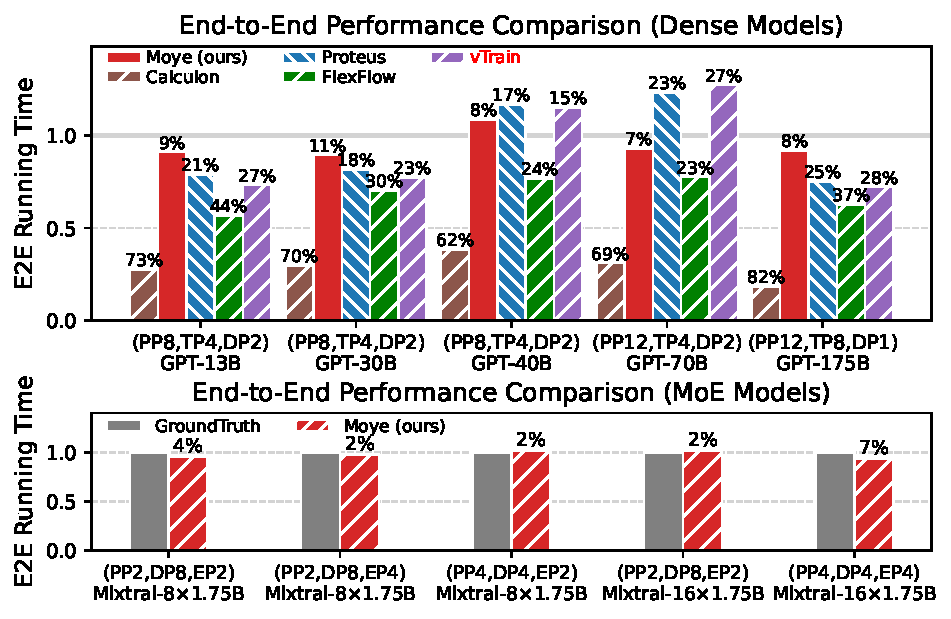
\includegraphics[width=1\linewidth]{figures/evaluation/NEW_end_to_end_normalized.pdf}
    \caption{\yc{End-to-end training step time comparison on dense and MoE models (up to 96 H800 GPUs). 
    All results are normalized to ground truth ($y{=}1.0$/gray bars). 
    Numbers above bars denote prediction error. Baseline systems do not support MoE simulation.}}
    \vspace{-0.2em}
    \label{fig:end_to_end} 
\end{figure}

\noindent\textbf{Accuracy.} 
We evaluate the end-to-end accuracy of \sys on H800 clusters of varying scales using Megatron-LM. 
As shown in Figure~\ref{fig:end_to_end}, \sys consistently achieves high fidelity across diverse parallelism configurations. 
For 96-GPU scenarios, the prediction error is 7\% for GPT-70B ($12\times4 \times2$) and 8\% for GPT-175B ($12\times8\times1$). 
In contrast, baseline simulators deviate significantly: Proteus and FlexFlow show errors exceeding 25\%, while Calculon is overly optimistic (error $>$69\%) due to its reliance on ideal analytical models. 
\sys also attains high accuracy on MoE models, with an average error of 3.4\%. 
Across models, \sys achieves average errors of 4.5\% and 17.8\% for computation and communication operations. 
Its accuracy is further improved by modeling slowdown from overlapping kernels. 
In our settings here, computation--communication overlap accounts for 6.0\%--9.8\% of total step time, and simulating the overlap-induced slowdown improves end-to-end accuracy by 3.6\%--5.2\%. 
As training systems increasingly optimize for aggressive overlap \cite{deepep}, accurate slowdown prediction may become even more critical.
\yc{
\begin{figure}[t]
    \centering
    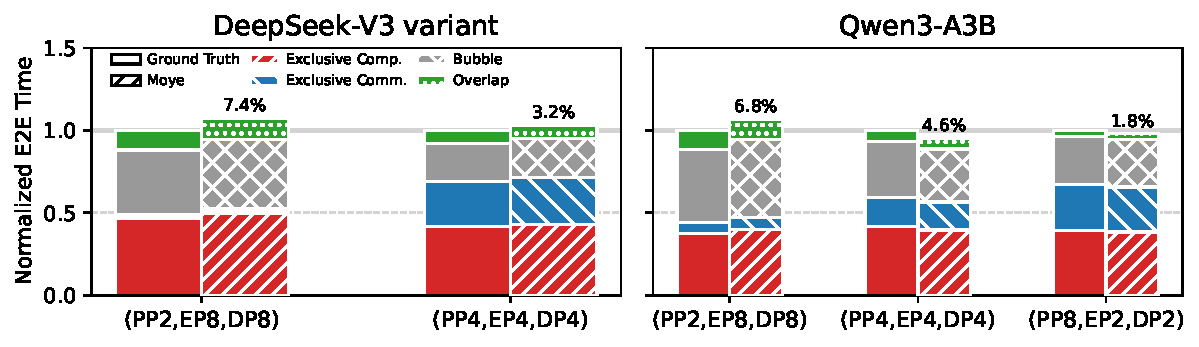
\includegraphics[width=1\linewidth]{figures/evaluation/latest_models_e2e_breakdown.pdf}
    \caption{\yc{End-to-end component breakdown for two latest MoE models in our H800 setup. Left: DeepSeek-V3 variant. Right: Qwen3-A3B. Each configuration shows a textured ground-truth bar and a colored stacked \sys bar decomposed into exclusive computation, exclusive communication, bubble, and overlap. Numbers above \sys bars denote absolute end-to-end prediction error. Proteus, FlexFlow, and Calculon are omitted because they do not support these latest models.}}
    \label{fig:end_to_end_latest_models}
\end{figure}

\noindent\textbf{Latest MoE models.}
We further evaluate \sys on two recently released MoE models, DeepSeek-V3 variant and Qwen3-A3B, in our H800 setup. These two models stress different MoE execution paths rather than merely larger parameter counts: Qwen3-A3B increases routing fan-out and expert diversity, whereas the DeepSeek-V3 variant combines MLA, group-limited routing, shared experts, and all-to-all expert communication. As shown in Figure~\ref{fig:end_to_end_latest_models}, other SOTA simulators cannot simulate these latest models, so we only compare \sys against ground truth. Across the five feasible configurations, \sys achieves an average end-to-end prediction error of 4.8\%, with a maximum error of 7.4\%. For Qwen3-A3B, the error ranges from 1.8\% to 6.8\%; for DeepSeek-V3 variant, it ranges from 3.2\% to 7.4\%. The overlap portion spans 3.5\%--12.8\% of total step time, while bubble remains a major contributor at 24.0\%--47.3\%. This breakdown indicates that the remaining gap is not dominated by expert communication alone, but also by compute-side phases and their interaction with overlap and pipeline bubbles.

\begin{table}[t]
\centering
\small
\renewcommand{\arraystretch}{0.95}
\begin{tabular}{@{}lcccc@{}}
\toprule
\textbf{Skew} & \textbf{Load} & \textbf{GT straggler} & \textbf{\sys straggler} & \textbf{Proxy err.} \\
\midrule
Balanced & 1.00 & 1.04 & 1.24 & 7.88\% \\
Moderate & 1.54 & 1.02 & 1.08 & 4.40\% \\
Strong & 3.00 & 1.08 & 1.22 & 6.64\% \\
\bottomrule
\end{tabular}
\caption{\yc{Controlled routing-skew stress test on the DeepSeek-V3 variant in our 8-GPU A800 setup ($PP{=}2$, $TP{=}1$, $EP{=}4$, $DP{=}4$), along the widely used no-token-dropping path. Load reports the hottest-to-median expert token count. The strongest skew regime increases the GT straggler ratio from the near-balanced 1.02--1.04 range to 1.08, while \sys keeps the critical-path proxy error within 4.4\%--7.9\%.}}
\label{table:moe_routing_skew}
\end{table}

\noindent\textbf{MoE routing-skew sensitivity.}
We further stress the DeepSeek-V3 variant with controlled expert-load skew while keeping the model architecture and parallel configuration fixed along the widely used no-token-dropping path. The moderate-skew case remains close to the balanced setting within system noise, but the strong-skew case makes a subset of EP ranks dominate the critical path more clearly. \sys predicts this stressed regime with 6.64\% critical-path proxy error, showing that its MoE fidelity extends beyond near-balanced routing under controlled routing skew. Explicit capacity-factor extremes and token-dropping/capacity-aware admission control remain future work.
}


\yc{
\begin{figure}[t]
    \centering
    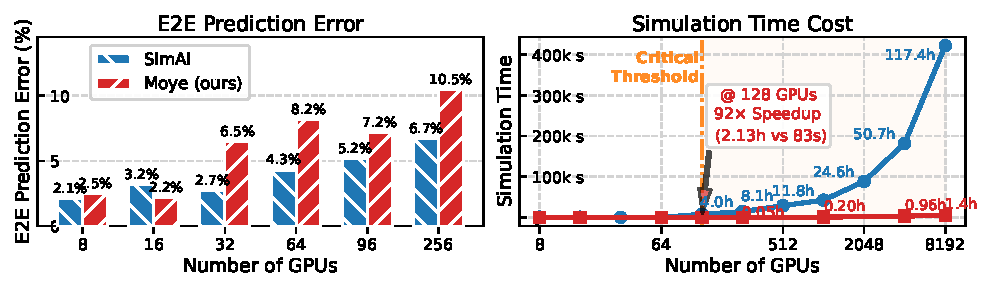
\includegraphics[width=1\linewidth]{figures/evaluation/simai_vs_moye.pdf}
    \caption{\yc{Comparison of \sys and SimAI on GPT-175B (H800 cluster, 3D parallelism). 
    Left: end-to-end prediction error across cluster scales. 
    Right: simulation time cost (log-log scale). 
    Beyond 128 GPUs, \sys achieves a 91.8$\times$ speedup over SimAI while maintaining comparable accuracy.}}
    \label{fig:simai_vs_moye}
    \vspace{-1em}
\end{figure}

\noindent\textbf{Comparison with packet-level simulator.}
We compare \sys against SimAI~\cite{SimAI2025NSDI}, a packet-level network simulator built on ns-3, on GPT-175B training across 8--8{,}192 H800 GPUs (Figure~\ref{fig:simai_vs_moye}).
In terms of accuracy, both simulators achieve comparable end-to-end prediction errors at small scales (2--3\% at 8--32 GPUs).
As the cluster grows, \sys's error increases moderately to 10.5\% at 256 GPUs, while SimAI remains at 6.7\%---a gap attributable to SimAI's finer-grained packet-level communication modeling.
However, the simulation time gap is dramatic.
At 128 GPUs, \sys completes in 83 seconds---a 91.8$\times$ speedup over SimAI's 7{,}655 seconds.
This advantage widens further at scale: at 8{,}192 GPUs, \sys finishes in 1.4 hours while SimAI requires over 117 hours.
For a design-space exploration sweeping 100 configurations on an 8{,}192-GPU cluster, \sys would complete in under 6 days, whereas SimAI would require over 1.5 years.
These results demonstrate that \sys offers a compelling accuracy--efficiency trade-off, making it practical for iterative what-if analysis at datacenter scale where packet-level simulation is prohibitively expensive.
}




% Ablation study
\yc{
\begin{figure}[t]
    \centering
    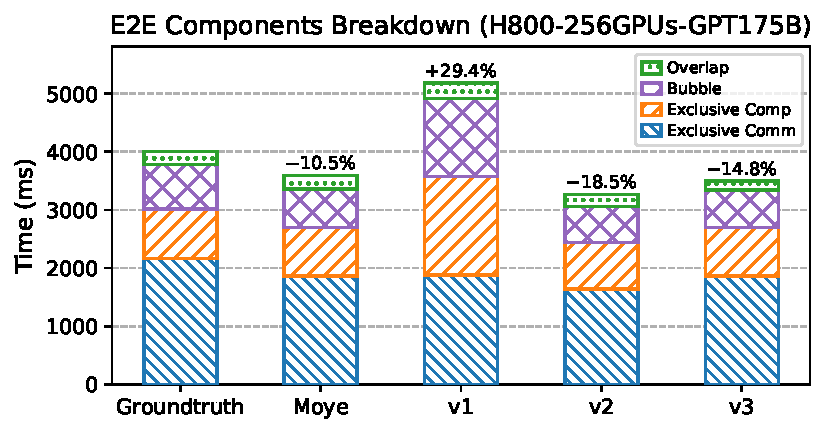
\includegraphics[width=0.75\linewidth]{figures/evaluation/component_breakdown_256gpu.pdf}
    \caption{\yc{Component breakdown of GPT-175B training step time on 256 H800 GPUs with 3D parallelism. Each bar decomposes the step time into exclusive computation, exclusive communication, bubble, and overlap. Numbers above bars denote end-to-end prediction error.}}
    \label{fig:ablation_breakdown}
    % \vspace{-1em}
\end{figure}

\noindent\textbf{Ablation study.}
To isolate the contribution of each key module, we perform an ablation study on GPT-175B (FP16) trained on a 256-GPU H800 cluster with 3D parallelism ($\text{PP}=16, \text{TP}=8, \text{DP}=2$).
We disable one module at a time and report the signed prediction error for each time component against ground truth (Figure~\ref{fig:ablation_breakdown} and Table~\ref{table:ablation}).

\begin{table}[t]
\centering
\small
\renewcommand{\arraystretch}{0.9}
\resizebox{\columnwidth}{!}{
\begin{tabular}{@{}lrrrrr@{}}
\toprule
\textbf{Variant} & \textbf{Excl. Comp.} & \textbf{Excl. Comm.} & \textbf{Bubble} & \textbf{Overlap} & \textbf{End-to-End} \\
\midrule
\sys (Full)            & $-$2.2\%   & $-$14.0\%  & $-$13.2\%  & $+$1.1\%   & $-$10.5\% \\
w/o Ex-situ Tracer (v1)   & $+$98.2\% & $-$13.0\%  & $+$75.0\%  & $+$21.1\%   & $+$29.4\% \\
w/o White-box Comm. (v2)    & $-$6.3\%   & $-$24.4\%  & $-$19.0\%  & $-$6.8\%   & $-$18.5\% \\
w/o Slowdown Pred. (v3)     & $-$2.5\%   & $-$13.9\%  & $-$15.7\%  & $-$31.9\%  & $-$14.8\% \\
\bottomrule
\end{tabular}}
\caption{\yc{Ablation study on GPT-175B (256 H800 GPUs, 3D parallelism). Each column shows the signed prediction error of the corresponding time component relative to ground truth.}}
\label{table:ablation}
\vspace{-1em}
\end{table}

Removing the ex-situ computation profiler and substituting analytical FLOPS estimates inflates the exclusive computation error to $+$98.2\%, which cascades into $+$75.0\% bubble error and $+$29.4\% end-to-end deviation---the largest among all variants.
Replacing the white-box communication model with an $\alpha$-$\beta$ model increases the exclusive communication error from 14.0\% to 24.4\% and worsens end-to-end accuracy from 10.5\% to 18.5\%.
Disabling slowdown prediction degrades overlap estimation from $+$1.1\% to $-$31.9\% error, raising the end-to-end error by 4.3 percentage points.
These results confirm that all three modules contribute meaningfully to \sys's end-to-end fidelity.
}



\yc{
\noindent\textbf{Simulation cost.}
We investigate \sys's two time costs:
(1) profiling time cost, and
(2) simulation time cost, including initialization and execution, and excludes the one-time, reusable workload tracing cost. 
}
As detailed in Table~\ref{table:simulation_cost}, \sys is highly efficient across training scenarios. For DDP, simulation is consistently fast, averaging about 10 seconds. The advantage is more pronounced for complex 3D parallelism; by leveraging its white-box communication model, \sys simulates a 128-GPU setup in 83 seconds—a 91.8x speedup over packet-level simulators like SimAI (7655s). This efficiency scales to large configurations, enabling the simulation of one step of an 8,192-GPU cluster in $<$1.4 hours.
For a typical design-space exploration over 100 training configurations on such a system, \sys would complete all simulations in under 6 days.
At this scale, the much higher per-configuration cost of packet-level network simulation (like SimAI) would push turnaround time to 1.5 years.



% table1
\begin{table}[t]
\centering
\small
\renewcommand{\arraystretch}{0.8}
\resizebox{\linewidth}{!}{
\begin{tabular}{ccccccccc}
\toprule
\multirow{2}{*}{\#GPUs} & \multicolumn{4}{c}{\textbf{VGG19}} & \multicolumn{4}{c}{\textbf{GPT 13B$\sim$175B}} \\ \cmidrule(lr){2-5} \cmidrule(lr){6-9}
                        & \textbf{Init.} & \textbf{Execution} & \textbf{Sim. Total} & \textbf{Trace} & \textbf{Init.} & \textbf{Execution} & \textbf{Sim. Total} & \textbf{Trace} \\ \midrule
256                     & 0.4            & 10.3           & 10.7           & \yc{18.2}      & 8.4             & 159.2          & 167.6          & \yc{1350.2}           \\
1024                    & 0.3            & 9.7            & 10.0           & \yc{18.5}      & 35.9            & 682.8          & 718.7          & \yc{1926.7}           \\
4096                    & 0.4            & 10.2           & 10.6           & \yc{17.8}      & 149.9           & 3307.8         & 3457.7         & \yc{2688.3}           \\
8192                    & 0.3            & 10.3           & 10.5           & \yc{18.3}      & 374.7           & 4602.2         & 4976.9         & \yc{3498.2}           \\ \bottomrule
\end{tabular}}
\caption{\yc{The simulation time costs of \sys in seconds. VGG19 is trained using the DDP mode, while GPT models (ranging from 13B to 175B) are trained using 3D parallelism.}}
\label{table:simulation_cost_old}
% \vspace{-2em}
\end{table}




\subsection{Computation and Memory Usage Simulation}
\label{subsec:workload_perf}

\noindent We evaluate \sys's accuracy in simulating computation workloads on both H800 and A800 clusters, using VGG19 (with DeepSpeed), GPT-13B and Mixtral-8×1.75B (both with Megatron-LM) under various PP/EP configurations. 

\noindent\textbf{Accuracy.} \sys reconstructs the computation workload by tracing all computational \ops and reproducing their execution sequence based on the \wg. Per-GPU \op running times are derived through \sys's \extractor without requiring a full-scale deployment. 
As shown in Figure~\ref{fig:comp_h}, \sys achieves a maximum overall error of 8.31\%. In contrast, while \bs and \ff maintain relatively low error rates for VGG19 under DeepSpeed (8.6\% and 17.81\%, respectively), their errors escalate dramatically for GPT-13B under Megatron-LM, reaching 91.53\% and 109.14\%, respectively.
The root cause of this discrepancy is that Proteus and FlexFlow rely heavily on standard PyTorch \ops, failing to incorporate the custom fused \ops that frameworks like Megatron-LM employ for performance optimization. 
Such specialized \ops cannot be accurately modeled without extracting their runtime characteristics directly from the target training framework (as we disccusion in~\cref{sec:motivation}). 
Calculon overestimates computation time in an overly idealized manner (error rate $>400\%$), because its modeling relies on hardware's analytical FLOPS values, which severely deviate from real hardware execution.
By precisely tracing, \sys captures the actual \op behaviors and achieves substantially higher accuracy.

\begin{figure}[t] 
    \centering 
    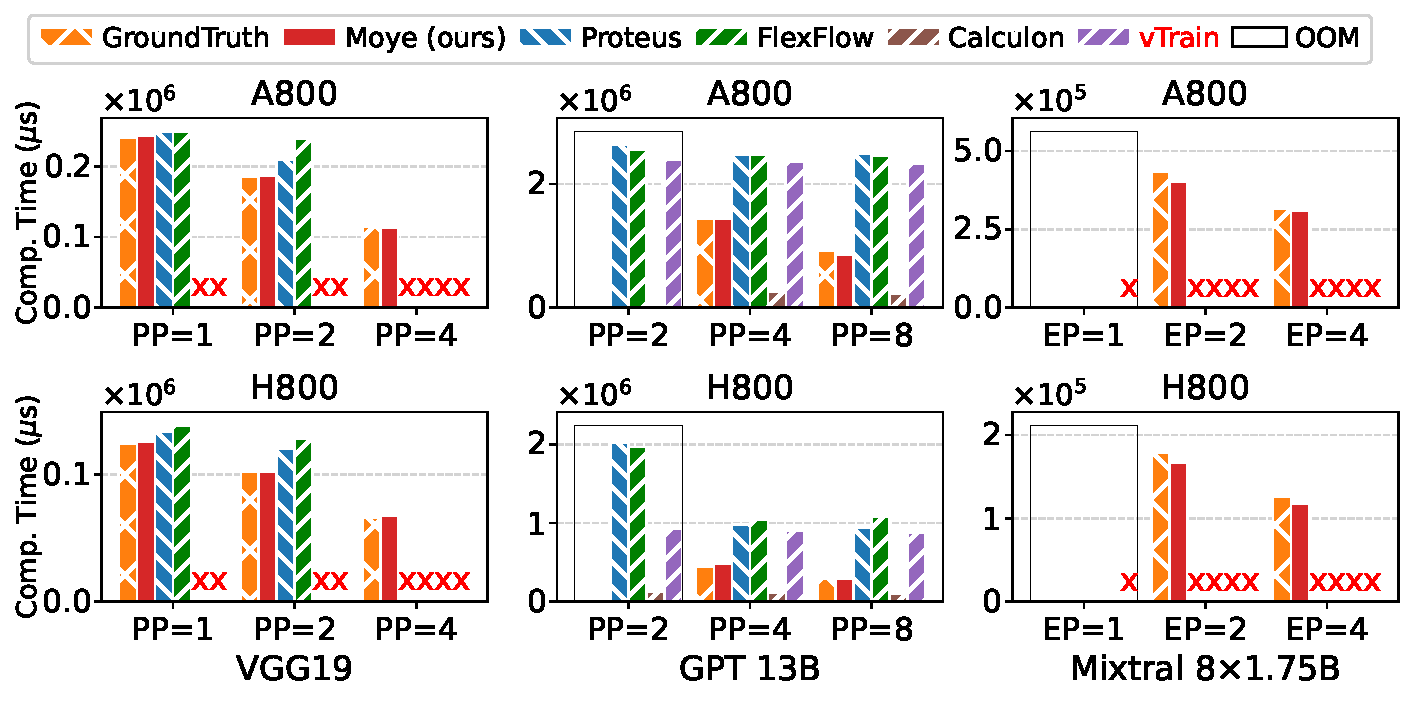
\includegraphics[width=1\linewidth]{figures/evaluation/comp_h800_a800_with_vtrain.pdf} 
    \caption{\yc{
        Computation times of various workloads on A800 and H800 clusters under different parallelization settings. Crosses denote cases not supported by the baselines, while squares mark configurations that encountered OOM errors during real execution.
    }}
    \label{fig:comp_h}
    \vspace{-2.2mm}
\end{figure}

\begin{figure}[t] 
    \centering 
    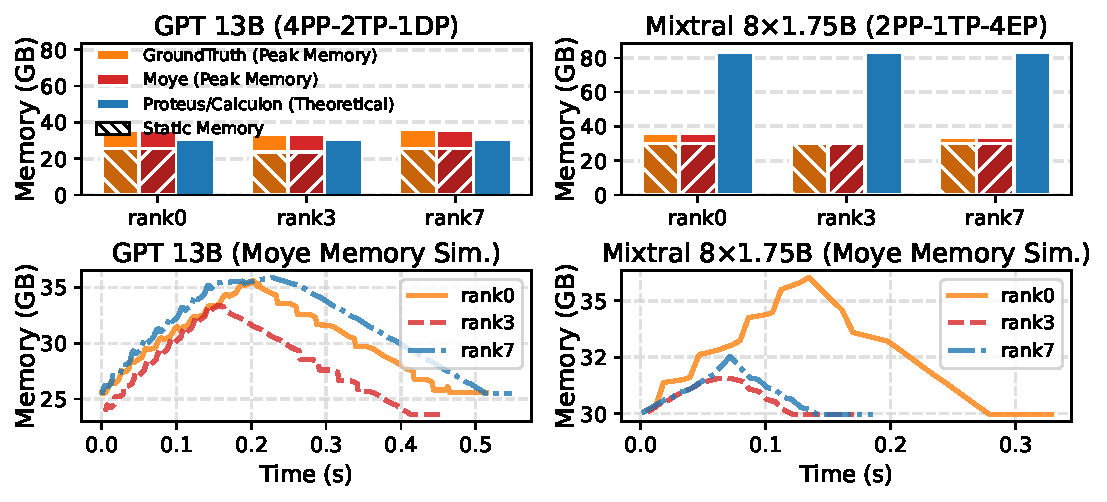
\includegraphics[width=1\linewidth]{figures/evaluation/memory_analysis_final.pdf} 
    \vspace{-2em}
    \caption{
        Validation of Moye's GPU memory simulation for GPT-13B and Mixtral-8$\times$1.75B on our 8-GPU A800 cluster (8 ranks), showing three representative ranks.
        It demonstrates Moye's ability to capture dynamic per-rank memory usage within a training step (excluding communication time). We set num\_micro\_batch=micro\_batch\_size=1 here.
    }
    \label{fig:memory}
    \vspace{-3mm}
\end{figure}

\vspace{0.1em}
\noindent\textbf{Generality.}
\sys is the only high-fidelity simulator that supports MoE workloads (error $<6\%$, Figure~\ref{fig:comp_h}). 
None of the baselines can handle MoE models.
Even for CNNs, Proteus and FlexFlow fail on certain configurations (e.g., VGG19 at PP=4) due to their reliance on manual, pre-hardcoded workload construction. 
In contrast, \sys supports simulations across a wide range of training design spaces. 
We further demonstrate its scalability via an ex-situ simulation of 8,192 GPUs in \cref{sec:usecase}.

\vspace{0.1em}
\noindent\textbf{GPU Memory usage.}
\sys supports high-fidelity GPU memory usage simulation through ex-situ profiling.
Figure~\ref{fig:memory} (upper) shows the peak memory usage (including both static and dynamic components), where \sys achieves nearly 100\% accuracy on GPT-13B and Mixtral-8$\times$1.75B for different ranks.
In contrast, analytical methods can result in 18.0\% error for GPT-13B, and for MoE models (Mixtral-8$\times$1.75B), the error even increase to 2.58$\times$ (a gap of 51 GB).
\sys can also reflect dynamic GPU allocation behavior during training, as shown in Figure~\ref{fig:memory} (lower)—a capability absent in existing simulators.
We believe this ability can help engineers identify potential optimization opportunities.

\begin{figure}[t] 
    \centering 
    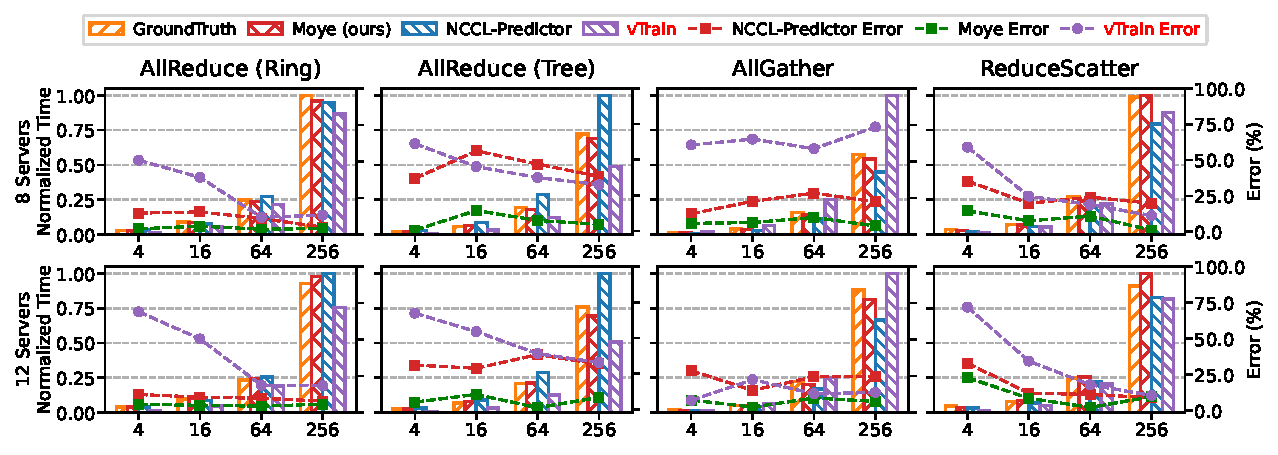
\includegraphics[width=1\linewidth]{figures/evaluation/inter_nccl.pdf} 
    \vspace{-.5cm}
    \caption{\yc{Running time and prediction error for inter-server CC kernels on H800 GPUs across varying tensor sizes and cluster scales. Each subplot is normalized relative to the operation with the longest running time.}}
    \label{fig:inter_nccl}
    \vspace{-1.2em}
\end{figure}

\subsection{Communication Simulation}
\label{subsec:allreduce_perf}

\noindent We now evaluate the effectiveness of \sys's communication simulation, comparing it against NCCL-Predictor~\cite{nccl}, the underlying communication model used by both \bs and \ff. NCCL-Predictor leverages parameters tuned from production experience and employs an ${\alpha-\beta}$ model~(\cref{subsec:challenges}).

\noindent\textbf{Accuracy.}  
Figures~\ref{fig:inter_nccl} show the prediction accuracy of collective communication across message sizes (4MB-256MB) and cluster scales. 
\sys consistently outperforms NCCL-Predictor, with average errors of 12.6\% and 13.8\% on 8- and 12-server H800 clusters, improving upon NCCL-Predictor by 29.6\% and 19.4\%, respectively.
\fx{Here, for 8- and 12-server clusters we set the scaling factor $c_{\mathrm{scale}}(N)$ to 1.023 and 1.063, respectively.}
The gap is smallest on ring-based \ar (4.2\%), where NCCL's heavy optimizations align well with the ${\alpha-\beta}$ model. 
For other patterns---especially tree-based \ar---\sys achieves much higher accuracy, reducing errors by up to 33.5\%.  

These improvements stem from \sys's profiling-based white-box model, which captures bandwidth utilization and synchronization overheads that NCCL-Predictor's simplified assumptions overlook. 
As a result, \sys maintains consistent accuracy for both small and large messages, whereas NCCL-Predictor suffers average errors of 27.6\% on 4MB and 16MB inputs.  
Finally, \sys's white-box design also accelerates simulation speed, as shown in~\cref{subsec:overall_perf}.
\yc{We further evaluate \sys on the \texttt{all-to-all}. As shown in Figure~\ref{fig:alltoall_error}, \sys achieves an average error of 13.6\% across 1- and 2-server H800 configurations, compared to 25.8\% for the $\alpha$-$\beta$ model. Since expert dispatch/combine in our Qwen3-A3B and DeepSeek-V3-style workloads is instantiated as \texttt{all-to-all}, this result directly validates \sys's communication model on the dominant MoE-specific collective, rather than only on dense-model traffic.}

\begin{figure}[t]
    \centering
    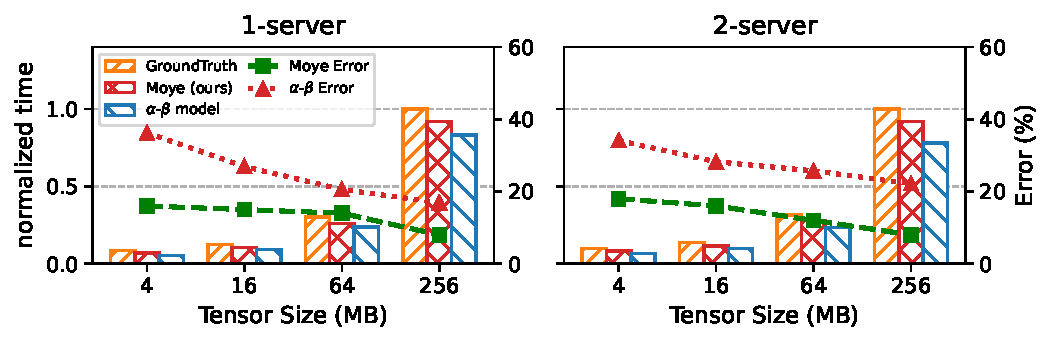
\includegraphics[width=.75\columnwidth]{figures/evaluation/alltoall_error_compare.pdf}
    \vspace{-0.6em}
    \caption{\yc{\sys's all-to-all running time prediction on H800 clusters.}}
    \label{fig:alltoall_error}
    % \vspace{-1em}
\end{figure}

\begin{table}[t] 
    \centering
    \small
    \renewcommand{\arraystretch}{0.8}
    \resizebox{\columnwidth}{!}{ 
        \begin{tabular}{@{}llllllll@{}}
            \toprule
            Tensor size (MB)           & 4      & 8       & 16    & 32      & 64      & 128     & 256     \\
            Chunk size ($10^3$ bytes)  & 18     & 36      & 72    & 72      & 72      & 144     & 288     \\ \midrule
            \begin{tabular}[c]{@{}l@{}}Intra-server \\ Round trip ($\mu$s) \end{tabular} & 57.43  & 64.36  & 73.62 & 74.61   & 77.46   & 75.55   & 99.23   \\ \midrule
            \begin{tabular}[c]{@{}l@{}}Inter-server \\ Round trip ($\mu$s) \end{tabular} & 54.3   & 72.32  & 106.73 & 112.9   & 111.25  & 174.2   & 278.98  \\ \midrule
            Reduce operation ($\mu$s) & 50.14  & 65.86  & 102.46 & 219.89  & 463.43  & 841.71  & 1657.72 \\ \bottomrule
        \end{tabular}}
    \caption{The breakdown of \sys's \ar running time, profiled in the H800 cluster using 32 GPUs.}
    \vspace{-4mm}
    \label{table:allreduce_param}
\end{table}

\noindent\textbf{Breakdown analysis.}
Table~\ref{table:allreduce_param} reports the breakdown of \ar runtime on a 32-GPU H800 cluster, separating intra-server latency, inter-server latency, and reduction computation across tensor sizes. 
Intra-server round-trip time increases moderately with tensor size (57.4~\textmu s at 4MB to 99.2~\textmu s at 256MB), reflecting the overhead of scheduling more thread blocks for larger chunks. 
Inter-server round-trip time shows a similar trend, growing to 279~\textmu s at 256MB. 
Reduction computation dominates at large tensors, scaling nearly linearly from 50.1~\textmu s (4MB) to 1658~\textmu s (256MB). 
These results demonstrate that \sys accurately captures both communication and computation overheads across varying message sizes. 




\subsection{Slowdown Prediction} 
\label{subsec:interference_perf}

\begin{figure}[t]
    \centering 
    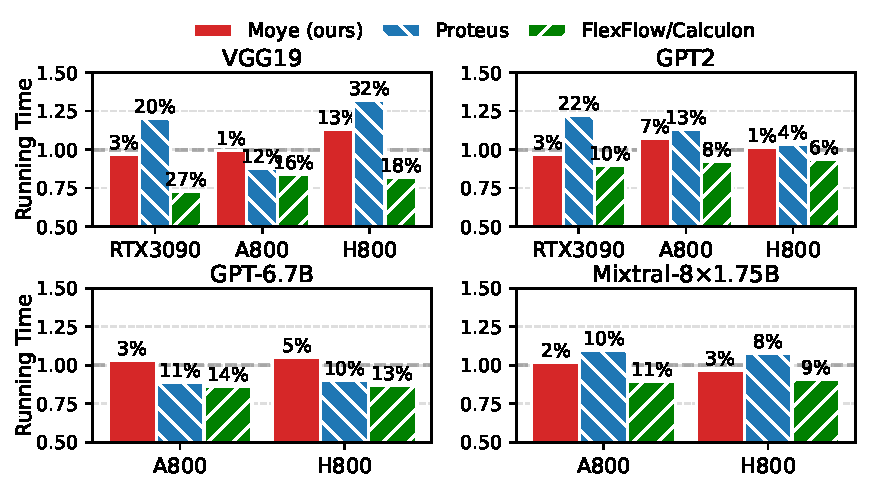
\includegraphics[width=0.95\linewidth]{figures/evaluation/model_wise_overlap_normolized2.pdf} 
    \vspace{-1em}
    \caption{
        Normalized model-wise computation time on H800, A800, and RTX3090 GPUs. 
        \sys (prediction-based) is compared against Proteus (fixed-parameter slowdown modeling) and FlexFlow/Calculon (no slowdown modeling). 
        Numbers above bars denote prediction error relative to ground truth (gray line at $y{=}1.0$).
    }
    \label{fig:model_wise_overlap}
\end{figure}

\begin{table}[t]
    \centering
    \small
    \renewcommand{\arraystretch}{0.85}
    \resizebox{0.85\columnwidth}{!}{
        \begin{tabular}{@{}llcccc@{}}
        \toprule
        Solution        & GPU & 5\% Error & 10\% Error & 15\% Error & RMSE \\ \midrule
        \sys     & \multirow{2}{*}{\centering 3090} & 61.48\% & 73.62\% & 76.52\% & 1.0935 \\
        Proteus         &                                   & 8.52\%  & 13.62\% & 19.28\% & 1.4953 \\ \midrule
        \sys      & \multirow{2}{*}{\centering A800}  & 61.03\% & 69.82\% & 75.01\% & 0.7147 \\
        Proteus         &                                   & 59.04\% & 65.45\% & 70.51\% & 1.5170 \\ \midrule
        \sys     & \multirow{2}{*}{\centering H800}  & 43.18\% & 51.59\% & 57.73\% & 0.5626 \\
        Proteus         &                                   & 34.78\% & 37.36\% & 40.18\% & 1.5493 \\ \bottomrule
        \end{tabular}}
    \caption{Fraction of cases where the slowdown prediction error is within the given error range.}
    \label{table:performance_comparison}
    \vspace{-1em}
\end{table}

\noindent Most simulators overlook the performance slowdown caused by kernel overlap. We compare \sys with \bs, the only baseline known to model this effect, which does so using a simple heuristic based on GPU architecture and model type.

\noindent\textbf{Prediction accuracy.}  
We evaluate slowdown prediction on $\sim$10,000 kernels (Table~\ref{table:performance_comparison}). 
\sys consistently outperforms the baseline heuristic, especially on data-center GPUs. 
On the H800, 57.7\% of predictions fall within 15\% error, compared to 40.2\% for the baseline, and the RMSE is nearly 3$\times$ lower (0.56 vs.\ 1.55). 
Similar gains hold on the A800, while on consumer-grade RTX 3090 GPUs, \sys again shows substantially lower error across all metrics. 

\noindent\textbf{Model-wise evaluation.} 
We further evaluate the impact of slowdown-aware modeling on training simulation accuracy across representative models. 
Experiments are conducted on modern training setups that already incorporate computation--communication overlapping: VGG19 and GPT2 with PyTorch DDP, GPT-6.7B with Megatron-LM 3D parallelism, and Mixtral-8$\times$1.75B with Flux, which enables fine-grained GroupedGEMM overlap. 
We slightly adjust model parameters so that overlapped kernels account for more than 25\% of execution time in all cases. 
Compared to baselines that ignore slowdown effects (FlexFlow and Calculon), incorporating slowdown improves the accuracy of simulating the computation portion by about 4\% on average. 
At the model level, \sys achieves the lowest prediction error across all tested architectures: 2--5\% on average, compared to 8--23\% for Proteus and 10--37\% for FlexFlow/Calculon (Figure~\ref{fig:model_wise_overlap}). 
These results highlight that accurate slowdown prediction is essential for faithfully modeling modern training workloads with heavy overlap. 
